\documentclass[11pt]{article}

\usepackage{blindtext}
\usepackage[pdftex]{graphicx}
\usepackage{fancyhdr}
\usepackage[margin=.8in]{geometry}
\usepackage[hang]{footmisc}
\usepackage{lipsum}
 \usepackage[flushleft]{threeparttable}
 \usepackage{tabularx} 
\usepackage{apacite}
\usepackage{float}
\usepackage{caption}
\usepackage{subcaption}
\usepackage{amsmath}
%\pagestyle{headings}
%\fancyhf{}
%\rhead{djfklas}
%\lhead{dkjfalj}
%\rfoot{ Page \thepage}
\usepackage{breqn}
\usepackage{titlesec}
\usepackage[labelfont={bf}]{caption}
%\usepackage{hyperref}
\usepackage{setspace}
\interfootnotelinepenalty=10000
\usepackage{arydshln}
\usepackage{rotating}
\usepackage{amsfonts}
\usepackage{bbm}
\usepackage{changepage}
\usepackage{pdflscape}
\newcommand{\etal}{\textit{et al}. }
\doublespacing
\newcolumntype{Y}{>{\centering\arraybackslash}X}

\def\sym#1{\ifmmode^{#1}\else\(^{#1}\)\fi}

\rfoot{ Page \thepage}


\begin{document}

\section{Border Effects Using PATH Stops}

The Port Authority Trans-Hudson (PATH) is a rapid transit system that runs between New Jersey and New York City 24 hours a day 7 days a week. This system is the primary transit link between Manhattan and neighboring New Jersey communities. It carries over 200,000 passengers daily. Figure 1 depicts the restaurants in Manhattan and the neighboring New Jersey area and their relation to the PATH railway stops. I now use these railway stops to estimate border effects using a secondary measure of distance-- driving minutes to a PATH stop. The following statistical model (model (3) from the full paper) will be used:
\begin{equation}
\begin{split}
\Delta \ln (p_{j,Oct16-Apr17})  = & \alpha_0 + \alpha_1  \mathbbm{1}(NY=1)  \\
& + \alpha_2 D_{j} + \alpha_3[D_j * \mathbbm{1}(NY=1)]  + \epsilon_{j}, 
\end{split}
\end{equation}
Figure 2 displays a binned scatter plot of the relationship between distance to a PATH stop and change in price. The first subfigure uses the Yelp restaurants and the change in price prior to any minimum wage changes. The second subfigure also uses the Yelp data but depicts price changes over the period when there was an increase in minimum wage. The third subfigure uses Grubhub restaurants and depicts time changes over the full sample period. 

Tables 1 and 2 report estimates of the border effects. Table 1 includes all restaurants within 12 minutes of a PATH stop and Table 2 includes all restaurants within 8 minutes of the border. For restaurants within 12 minutes of the border the estimated relationship between distance to a PATH stop and price change is insignificant for restaurants in both areas and in both datasets. The relationship for restaurants in NYC ($\alpha_2 + \alpha_3$) is much smaller than the estimates using driving distance to the border and negative. For restaurants within 8 minutes of a PATH stop, the relationship between distance and price change is estimated to be positive but relatively small and insignificantly estimated for restaurants in NYC. For restaurants in NJ ($\alpha_2$) the relationship is positive, significant, and relatively large in magnitude. 

\section{Figures}

\begin{figure}[H]
\centering
\caption{NYC-NJ Restaurants and PATH Stops}
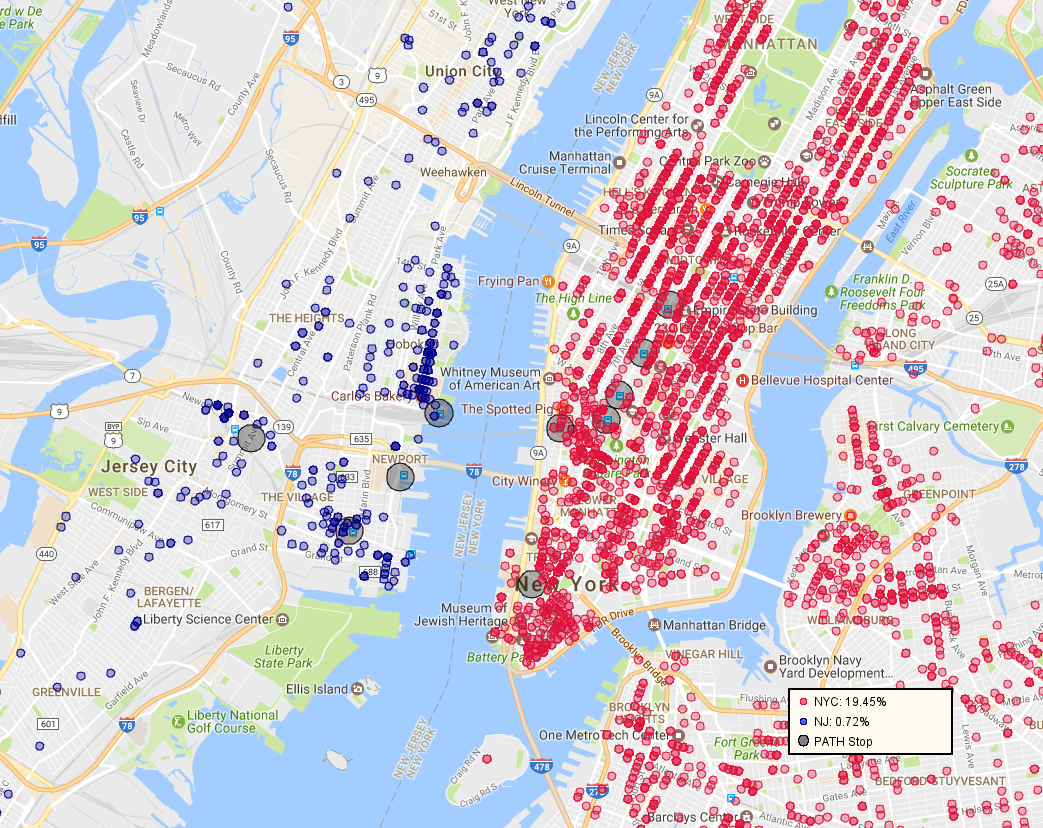
\includegraphics[width=6in]{pathmap.png}


{\footnotesize \raggedright \underline{Notes:} Each data point represents a restaurant in the Yelp dataset. Each PATH stop is the location where The Port Authority Trans-Hudson Rail System picks up pedestrians.   \par}
\end{figure}

\newpage
\begin{figure}[H]
\centering
\caption{Binned Scatter Plots}
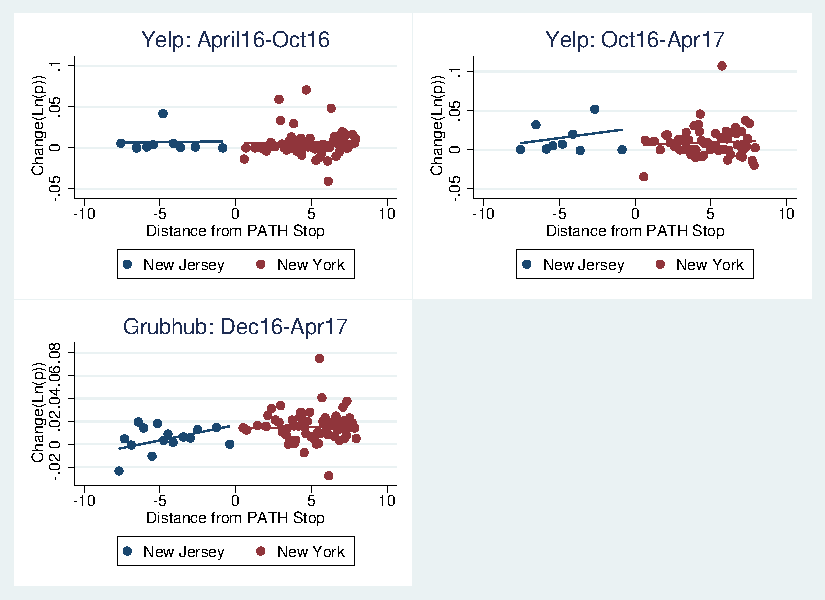
\includegraphics[width=6in]{path_plots.pdf}


{\footnotesize \raggedright \underline{Notes:}The figure shows the relationship between the change in price and the distance to the NYC- NJ border. Restaurants are binned into 80 quantiles. Distance is measured in driving minutes to the nearest PATH rail stop. The top two subfigures use Yelp data, where the first is prior to the minimum wage increases and the second is over the minimum wage increase time period. The bottom subfigure displays the relationship using Grubhub data over the minimum wage change time period. \par}
\end{figure}

\newpage

\section{Tables}

\begin{table}[H]
\centering
\caption{Border Effects: 12 Minutes}
\begin{center}
\begin{tabular}{lccccc}
\hline Source & \multicolumn{2}{c}{Yelp} & Grubhub &  & \\
 & (1) & (2) & (3) &  & \\
Comparison Area &   NJ    &   NJ    &   NJ    &  & \\
Time Frame & Oct16-Apr17 & Apr16-Oct16 & Dec16-Apr17 &  & \\
\hline  $ \mathbbm{1}(NY) \quad (\alpha_1) $  & -0.0183 & 0.0029 & 0.0118* &  & \\
  & (0.0203) & (0.0102) & (0.0071) &  & \\
 Distance $\quad (\alpha_2) $  & 0.0028 & -0.0005 & -0.0001 &  & \\
  & (0.0028) & (0.0014) & (0.0010) &  & \\
 Distance * $ \mathbbm{1}(NY) \quad (\alpha_3) $  & -0.0030 & 0.0003 & -0.0004 &  & \\
  & (0.0029) & (0.0015) & (0.0010) &  & \\
 Constant $\quad (\alpha_0) $  & 0.0284 & 0.0043 & 0.0053 &  & \\
  & (0.0192) & (0.0097) & (0.0065) &  & \\
\hline  $ \alpha_2 + \alpha_3 $  & -0.0003 & 0.0005 & -0.0005 &  & \\
  & (0.0009) & (0.0029) & (0.0004) &  & \\
\hline  $ N $  & 1564 & 1564 & 1639 &  & \\
\hline\end{tabular}\\
\begin{tiny}\ * $p<0$.1; ** $p<0$.05; *** $p<0$.01\end{tiny}\\
\end{center}

{\footnotesize \raggedright \underline{Notes:} 
The outcome variable is the percentage point change in price due to a 10 minute change in the distance of a restaurant to a path stop. The first column includes restaurants in the Yelp dataset within twelve minutes of the NYC - NJ border between October 2016 and April 2017. Column 2 includes these same restaurants but using the change in price from July 2016 to October 2016 as the outcome. Columns 4 and 5 include restaurants in the Grubhub dataset. Column 4 reports effects on the NYC-NJ border. \par
}
\end{table}

\begin{table}[H]
\centering
\caption{Border Effects: 8 Minutes}
\begin{center}
\begin{tabular}{lccc}
\hline Source & \multicolumn{2}{c}{Yelp} & Grubhub\\
 & (1) & (2) & (3)\\
Comparison Area &   NJ    &   NJ    &   NJ   \\
Time Frame & Oct16-Apr17 & Apr16-Oct16 & Dec16-Apr17\\
\hline  $ \mathbbm{1}(NY) \quad (\alpha_1) $  & -0.0216 & -0.0022 & -0.0032\\
  & (0.0237) & (0.0161) & (0.0094)\\
 Distance $\quad (\alpha_2) $  & 0.0026 & 0.0002 & 0.0027*\\
  & (0.0043) & (0.0029) & (0.0016)\\
 Distance * $ \mathbbm{1}(NY) \quad (\alpha_3) $  & -0.0020 & -0.0002 & -0.0024\\
  & (0.0046) & (0.0031) & (0.0018)\\
 Constant $\quad (\alpha_0) $  & 0.0280 & 0.0082 & 0.0168**\\
  & (0.0224) & (0.0152) & (0.0083)\\
\hline  $ \alpha_2 + \alpha_3 $  & 0.0006 & -0.0003 & 0.0003\\
  & (0.0014) & (0.0062) & (0.0008)\\
\hline  $ N $  & 942 & 942 & 958\\
\hline\end{tabular}\\
\begin{tiny}\ * $p<0$.1; ** $p<0$.05; *** $p<0$.01\end{tiny}\\
\end{center}

{\footnotesize \raggedright \underline{Notes:} 
The outcome variable is the percentage point change in price due to a 10 minute change in the distance of a restaurant to a path stop. The first column includes restaurants in the Yelp dataset within twelve minutes of the NYC - NJ border between October 2016 and April 2017. Column 2 includes these same restaurants but using the change in price from July 2016 to October 2016 as the outcome. Columns 4 and 5 include restaurants in the Grubhub dataset. Column 4 reports effects on the NYC-NJ border.  \par
}
\end{table}


\end{document}